
\begin{minipage}[t]{0.62\textwidth}  % First column larger (65% of text width)
    \section{Education}

	\begin{tblr}{%
		colspec={ t{5.25cm} X[l,8] },  % Column specifications: first column with fixed width, rest flexible
		column{1} = {font=\fontsize{11}{12}\selectfont}, % 11pt font with 12pt line spacing for column 1 (bold)
		column{2} = {font=\fontsize{11}{12}\selectfont},           % 11pt font for column 2 (non-bold)
		column{3} = {font=\fontsize{11}{12}\selectfont},           % 11pt font for column 3 (non-bold)
		width=1.0\textwidth,
		colsep = 0.1pt,  % Adjust column spacing
		rowsep=0.001\baselineskip} % Adjust row spacing
	
	% Table contents
	\bfseries Ph.D. in Particle Physics & \CVevent{2024 (current)}{University of Calgary} \\
	\bfseries M.Sc. in Space Physics & \CVevent{2022 - 2023}{University of Calgary} \\
	\bfseries B.Sc. in Physics & \CVevent{2017 - 2021}{University of Calgary} \\
	\end{tblr}

\end{minipage}
\hspace{0.03\textwidth} 
\begin{minipage}[t]{0.3\textwidth}  % Second column smaller (30% of text width)
	
	\paragraph{ \ }
	\vspace*{-.25cm}
	\begin{tikzpicture}
		\begin{scope}
			\clip (0,0) circle (1.8cm);
			\node at (0, -0.25) {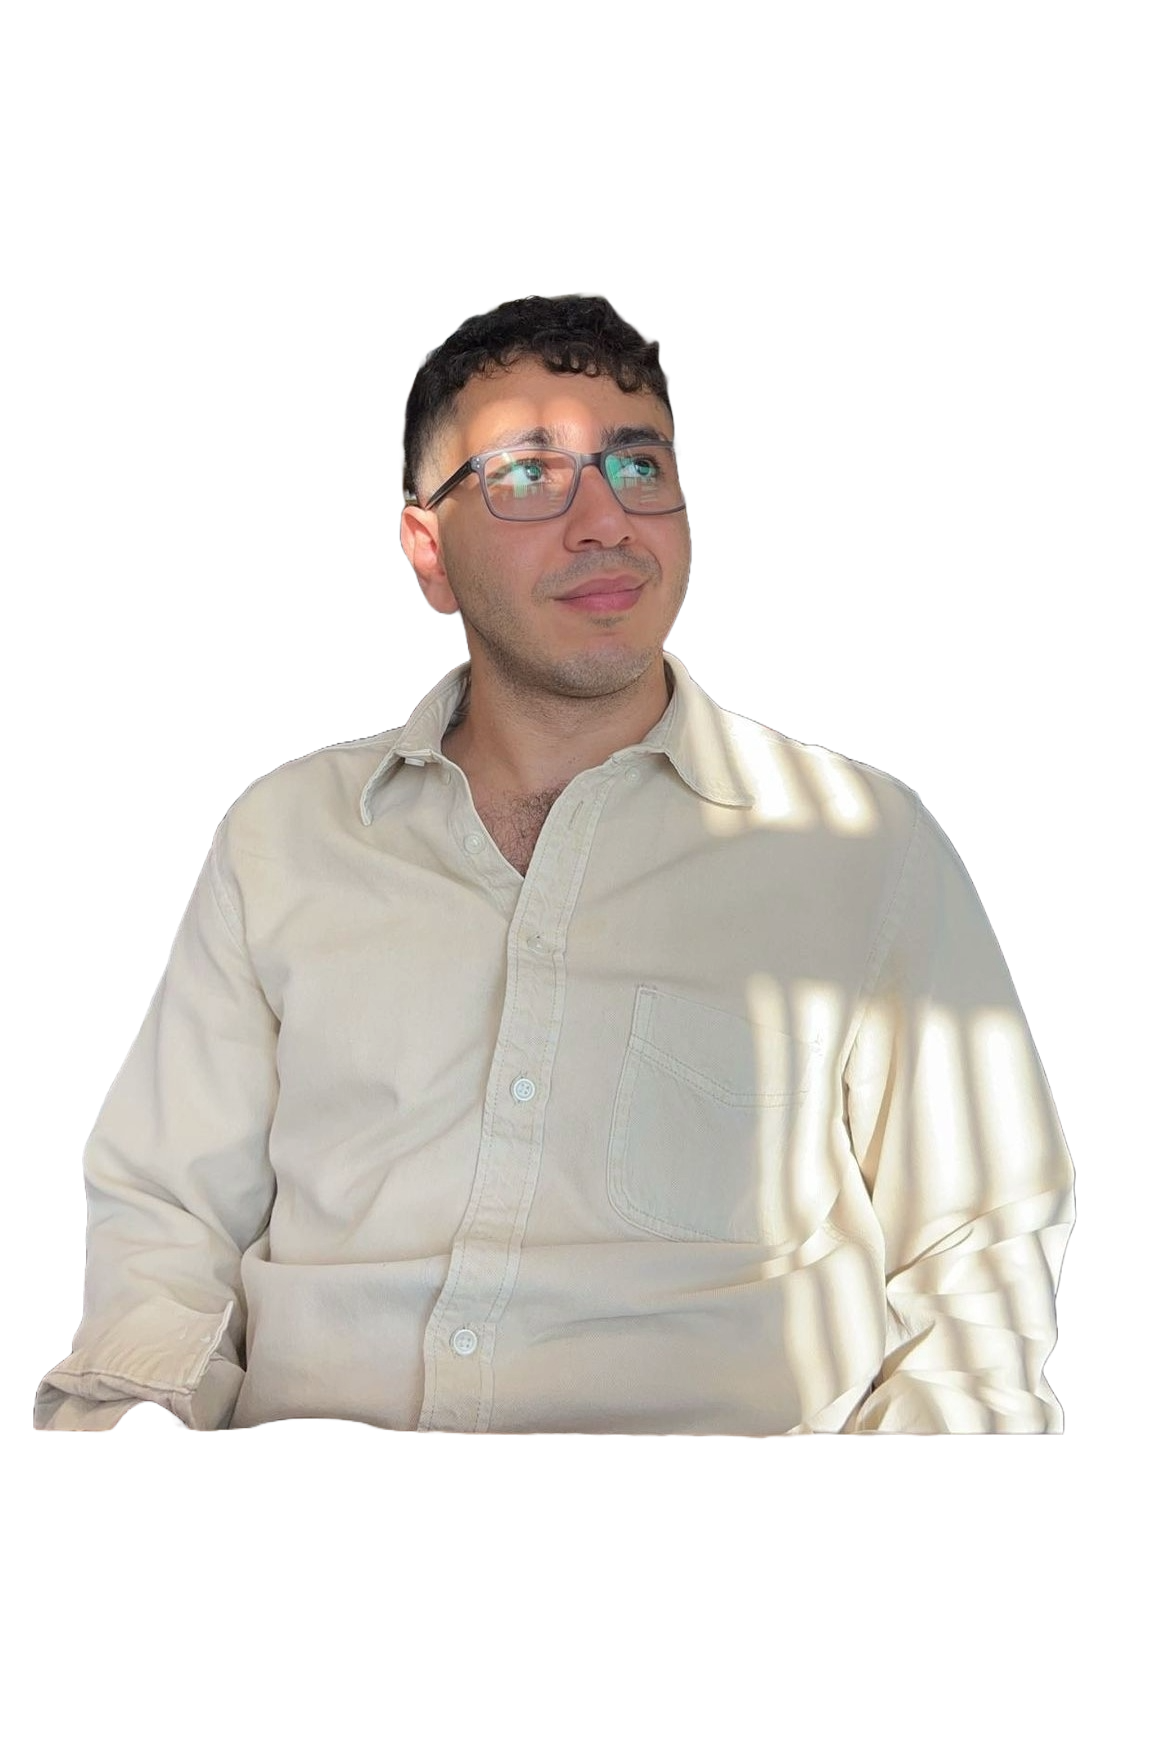
\includegraphics[width=3.5cm, height=5.75cm]{Img/no_bg_profile_1.png}};
		\end{scope}
		\draw[black] (0,0) circle (1.8cm); 
	\end{tikzpicture}
	\vspace*{-.25cm}

	% \begin{tikzpicture}
    %     % Clip the image into a circle and scale it to half the width of the first minipage (0.31\textwidth)
    %     \node[anchor=center, circle, minimum size=0.31\textwidth, clip] at (0,0)
    %         {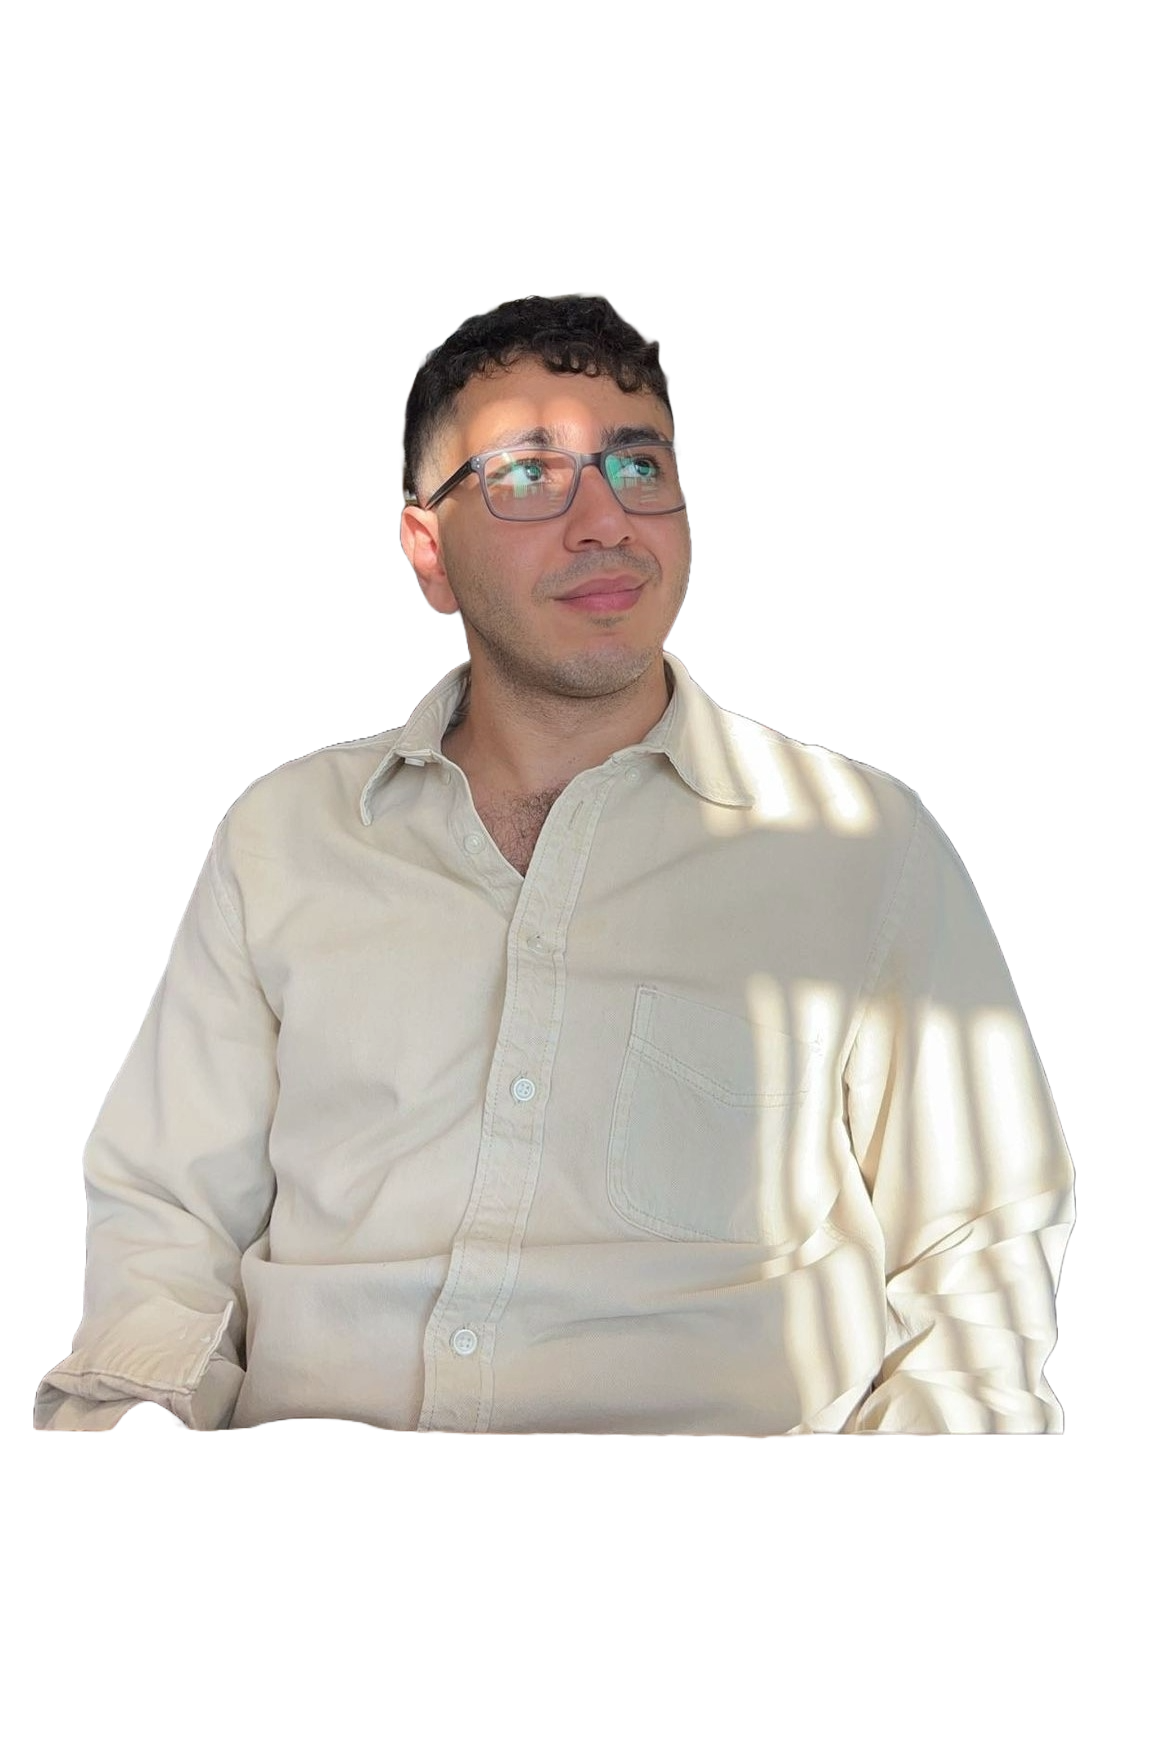
\includegraphics[width=0.31\textwidth]{Img/no_bg_profile_1.png}};
    % \end{tikzpicture}
	

	\section{Languages}
	\LngLvlCEFR{Arabic}{C2}
	\LngLvlCEFR{English}{C2}


	% \LngTextCEFR
\end{minipage}

\section{Publications}

\printbibliography[ heading=pubtype, type=thesis, title={\pubtitle{masterthesis}} ]

\printbibliography[ heading=pubtype, type=article, title={\pubtitle{article}} ]
\printbibliography[ heading=pubtype, type=report, title={\pubtitle{report}} ]

\newrefcontext[sorting=ydnt]
\printbibliography[ heading=pubtype, type=inproceedings, title={\pubtitle{conference}}]

\begin{Summary}{Skills}
	\underline{Programming:} \ \
	\veritem{Python}
	\veritem{Java}
	\veritem{JavaScript}
	\veritem{C++}
	\veritem{MATLab}
	\veritem{GNU Radio Companion}
	\veritem{PostgreSQL}
	\veritem{SQLite}
	\veritem{Django}
	\veritem{CSS}
	\veritem{HTML}
	\\ \\
	\underline{Hardware:} \ \
	\veritem{Software Defined Radios (SDR)}
	\veritem{Antennae}
	\veritem{Microcontrollers}
	\\ \\
	\underline{Modelling:} \ \
	\veritem{AutoCAD Inventor}
	\veritem{COMSOL Multiphysics}

\end{Summary}